\section{La recta}

Una recta $r$ queda determinada per qualsevol d'aquestes dades:

\begin{itemize}
\item Dos punts $P$ i $Q$, o equivalentment un punt $P$ i el vector director $\vec u = \overrightarrow{PQ}$.
\item Dos plans $\pi_1$ i $\pi_2$ no paral\textperiodcentered{}lels (la recta és la seva intersecció).
\item Un punt $P$ i un pla $\pi$ perpendicular a la recta.
\end{itemize}

La figura il\textperiodcentered{}lustra els tres casos:

\begin{figure}[H]
\centering
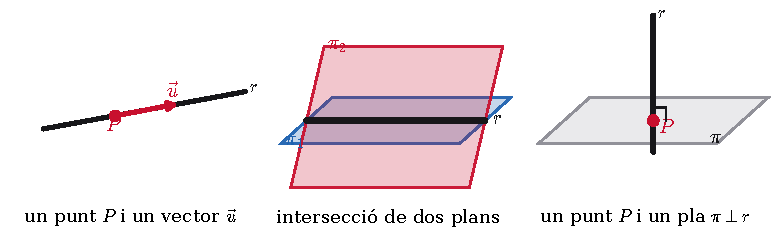
\includegraphics[width=372pt]{fig/m09_f17.pdf}
\caption{Tres maneres de determinar una recta a l'espai.}
\end{figure}

\subsection{Equació vectorial d'una recta}

Donat un punt $P(x_0, y_0, z_0)$ i un vector director $\vec u = (u_1, u_2, u_3)$:

\begin{equation*}
\vec x = \vec p + \lambda\,\vec u, \qquad \forall\lambda\in\mathbb{R}
\end{equation*}

\subsection{Equacions paramètriques d'una recta}

\begin{equation*}
\begin{cases} x = x_0 + \lambda\,u_1 \\ y = y_0 + \lambda\,u_2 \\ z = z_0 + \lambda\,u_3 \end{cases} \qquad \forall\lambda\in\mathbb{R}
\end{equation*}

\subsection{Equacions contínues d'una recta}

Aïllant $\lambda$ de les equacions paramètriques i igualant:

\begin{equation*}
\frac{x - x_0}{u_1} = \frac{y - y_0}{u_2} = \frac{z - z_0}{u_3}
\end{equation*}

\section{El pla}

Un pla $\pi$ queda determinat per qualsevol d'aquestes dades:

\begin{itemize}
\item Tres punts $P$, $Q$ i $R$ no alineats.
\item Un punt $P$ i dos vectors $\vec u$ i $\vec v$ linealment independents (vectors directors del pla).
\item Un punt $P$ i un vector $\vec n \neq \vec 0$ perpendicular al pla (vector normal).
\end{itemize}

\subsection{Equació vectorial d'un pla}

\begin{equation*}
\vec x = \vec p + \lambda\,\vec u + \mu\,\vec v, \qquad \forall\,\lambda,\mu\in\mathbb{R}
\end{equation*}

\subsection{Equacions paramètriques d'un pla}

\begin{equation*}
\begin{cases} x = x_0 + \lambda\,u_1 + \mu\,v_1 \\ y = y_0 + \lambda\,u_2 + \mu\,v_2 \\ z = z_0 + \lambda\,u_3 + \mu\,v_3 \end{cases} \qquad \forall\,\lambda,\mu\in\mathbb{R}
\end{equation*}

\subsection{Equació general (cartesiana) d'un pla}

S'obté desenvolupant el determinant de l'equació vectorial. La forma és:

\begin{equation*}
\begin{vmatrix} x - x_0 & u_1 & v_1 \\ y - y_0 & u_2 & v_2 \\ z - z_0 & u_3 & v_3 \end{vmatrix} = 0 \;\Longrightarrow\; Ax + By + Cz + D = 0
\end{equation*}

\section{Vector associat a un pla}

Donat el pla $\pi: Ax + By + Cz + D = 0$, el vector $\vec n = (A, B, C)$ és perpendicular al pla i s'anomena \textbf{vector normal} o \textbf{vector associat}.

\begin{figure}[H]
\centering
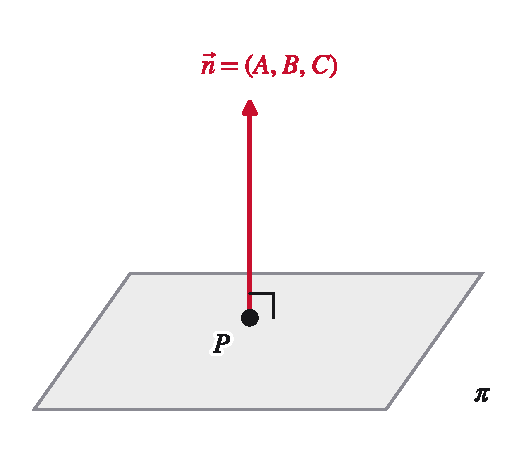
\includegraphics[width=248pt]{fig/m09_f18.pdf}
\caption{El vector normal $\vec n = (A, B, C)$ és perpendicular al pla $Ax + By + Cz + D = 0$.}
\end{figure}

\section{Recta determinada per dos plans}

La intersecció de dos plans no paral\textperiodcentered{}lels determina una recta:

\begin{equation*}
r: \begin{cases} Ax + By + Cz + D = 0 \\ A'x + B'y + C'z + D' = 0 \end{cases}
\end{equation*}

Perquè els dos plans determinin una recta cal que siguin no paral\textperiodcentered{}lels, és a dir, que els seus vectors normals $\vec n_1 = (A, B, C)$ i $\vec n_2 = (A', B', C')$ no siguin proporcionals. El vector director de la recta resultant és $\vec u = \vec n_1 \times \vec n_2$.

\section{Feix de plans}

\textbf{Definició:} El \textbf{feix de plans} és el conjunt de tots els plans que contenen (o passen per) una mateixa recta $r$. El vector normal de cadascun dels plans del feix és perpendicular a $r$.

Si la recta $r$ és la intersecció dels plans $\pi_1: A_1x + B_1y + C_1z + D_1 = 0$ i $\pi_2: A_2x + B_2y + C_2z + D_2 = 0$, qualsevol pla del feix es pot expressar com:

\begin{equation*}
\lambda\,(A_1x + B_1y + C_1z + D_1) + \mu\,(A_2x + B_2y + C_2z + D_2) = 0, \qquad (\lambda, \mu) \neq (0, 0)
\end{equation*}

\section{Complement: mètode per obtenir equacions}

\subsection{Recta per dos punts}

Per a la recta que passa per $A$ i $B$: es pren $A$ com a punt i $\vec d=\overrightarrow{AB}$ com a vector director.

\emph{Exemple:} Recta per $A(1,2,3)$ i $B(3,0,4)$. Vector director $\vec d=(2,-2,1)$.

\begin{equation*}
\begin{cases}x=1+2t\\y=2-2t\\z=3+t\end{cases}\qquad\Longleftrightarrow\qquad\frac{x-1}{2}=\frac{y-2}{-2}=\frac{z-3}{1}
\end{equation*}

\subsection{Pla per tres punts}

Es prenen dos vectors del pla, $\overrightarrow{AB}$ i $\overrightarrow{AC}$; el vector normal és el seu producte vectorial, i amb ell s'escriu $Ax+By+Cz+D=0$ imposant que passi per $A$.

\emph{Exemple:} Pla per $A(1,0,0)$, $B(0,1,0)$ i $C(0,0,1)$. $\overrightarrow{AB}=(-1,1,0)$ i $\overrightarrow{AC}=(-1,0,1)$, i

\begin{equation*}
\vec n=\overrightarrow{AB}\times\overrightarrow{AC}=(1,1,1)\;\Rightarrow\;x+y+z+D=0,\ \ A\in\pi\Rightarrow D=-1
\end{equation*}

El pla és $\pi:\ x+y+z-1=0$.

\emph{Alternativa:} $\begin{vmatrix}x-1&y&z\\-1&1&0\\-1&0&1\end{vmatrix}=0$ dóna el mateix pla.

\subsection{Passar d'una forma a una altra}

\textbf{De contínua a implícita} (dos plans). Se separen les igualtats de dues en dues.

\emph{Exemple:} $\dfrac{x-1}{2}=\dfrac{y+1}{-1}=\dfrac{z}{3}$.

\begin{itemize}
\item Primera i segona: $-(x-1)=2(y+1)\Rightarrow x+2y+1=0$.
\item Segona i tercera: $3(y+1)=-z\Rightarrow 3y+z+3=0$.
\end{itemize}

\begin{equation*}
r:\ \begin{cases}x+2y+1=0\\3y+z+3=0\end{cases}
\end{equation*}

\textbf{De implícita a paramètrica.} Es resol el sistema prenent una incògnita com a paràmetre.

\emph{Exemple:} $\begin{cases}x+y-z=1\\2x-y+z=2\end{cases}$. Sumant: $3x=3\Rightarrow x=1$. Llavors $y-z=0$; prenem $z=t$ i $y=t$.

\begin{equation*}
r:\ (x,y,z)=(1,0,0)+t\,(0,1,1)
\end{equation*}

\emph{Un cop tens un punt i un vector director, tens tot el que cal per al tema 10 i 11.}
